
%------------------------------------------------------------------------
\begin{frame}
	\frametitle{Aggregate Realizations}
	\begin{block}{Definition}
		An \textbf{aggregate realization} is a particular type of partial order $C$ in which, for any pair of pitch classes $a, b$, if $a$ and $b$ are incomparable in $C$, then the set of pitch classes that precede $a$ in $C$ is equal to the set of pitch classes that precede $b$ in $C$, and also the set of pitch classes that follow $a$ in $C$ is equal to the set of pitch classes that follow $b$ in $C$.
	\end{block}
	\begin{block}{Example}
		\begin{itemize}
			\item Aggregate realizations arise naturally from a total order in the sense that they belong to the set of all partial orders that are covered by said total order
			\item Aggregate realizations lead to a classification of partial orders, as well as to many musical applications
			\item An interesting compositional application of aggregate realizations is that of projecting a total order as a middle-ground entity
		\end{itemize}
	\end{block}
\end{frame}

%------------------------------------------------------------------------
\begin{frame}
	\frametitle{Aggregate Realization in Webern's \emph{Variations} Op.~27}
	\begin{figure}
		\centering
		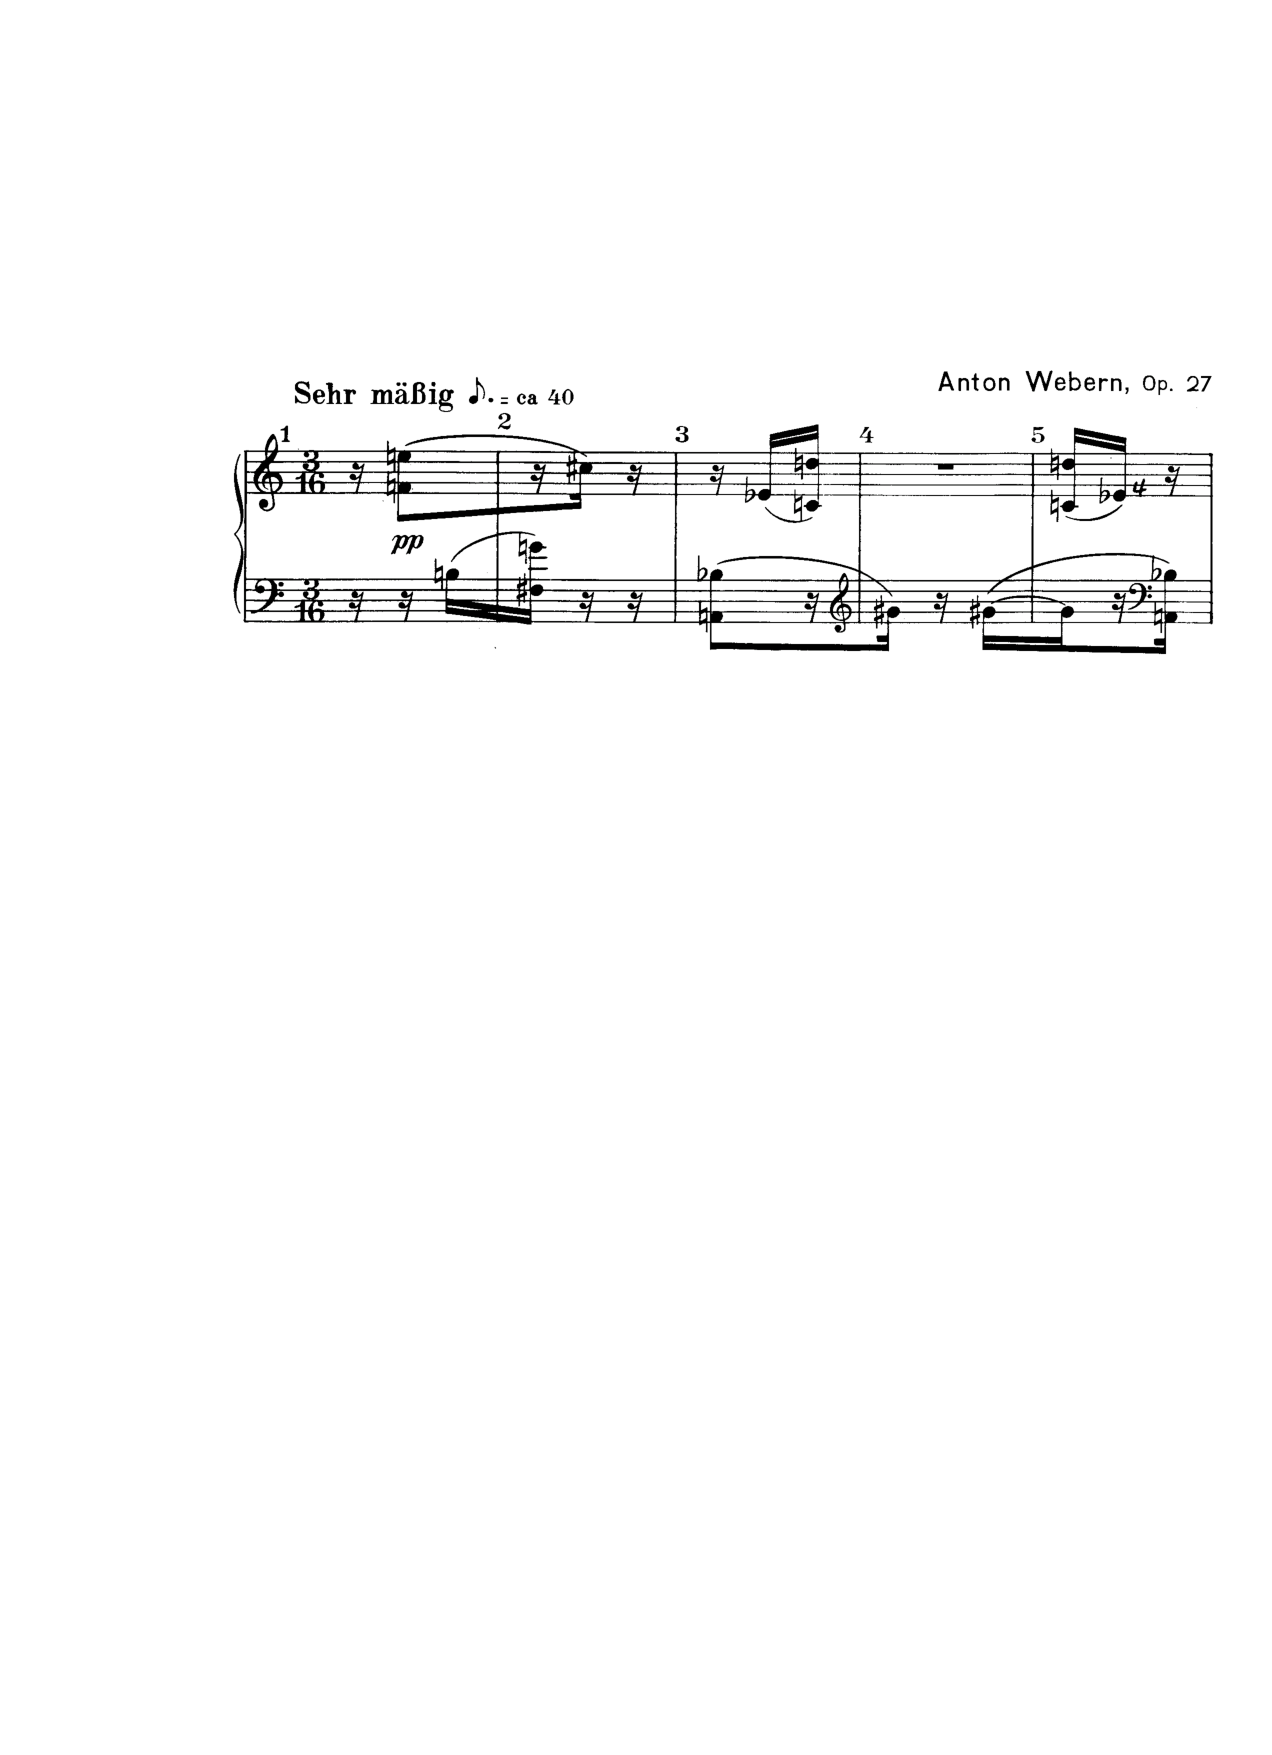
\includegraphics[width=\textwidth]{figures/webern1.pdf}
		\caption[Bars 1--7 in Webern's Op.~27]{The initial bars in Webern's Op.~27.}
	\end{figure}
\end{frame}

%------------------------------------------------------------------------
\begin{frame}[fragile]
	\frametitle{Aggregate Realization in Webern's \emph{Variations} Op.~27}
	\begin{figure}
		\centering
		\begin{adjustbox}{width=\textwidth}
		\begin{tikzcd}
			& E \arrow[dr] && G \arrow[dr] && B\flat \arrow[dr] && D \arrow[dr] & \\
			* \arrow[dr] \arrow[ur] && B \arrow[dr] \arrow[ur] && C\sharp \arrow[dr] \arrow[ur] && E\flat \arrow[dr] \arrow[ur] && G\sharp \\
			& F \arrow[ur] && F\sharp \arrow[ur] && A \arrow[ur] && C \arrow[ur] &
		\end{tikzcd}
		\end{adjustbox}
		\caption{An aggregate realization of the initial bars in Webern's Op.~27. At its very first presentation, the total order used to generate the piece cannot be discerned. Moreover, the partial order we are actually able to hear intercalates the total order's two hexachords, a procedure that can be construed as a form of derivation.}
	\end{figure}
\end{frame}

%------------------------------------------------------------------------
\begin{frame}
	\frametitle{Columnar Realizations}
	\begin{block}{Definition}
		A \textbf{columnar realization} is a set of disjoint row segments where the internal order of each segment is total, but all segments remain pairwise incomparable. We require that a columnar realization contain the free aggregate as a subset, so that we get all pitch classes belonging to a given base at each column.
	\end{block}
	\begin{block}{Example}
		\begin{itemize}
			\item The intersection of the set of all aggregate realizations with the set of all columnar realizations contains the set of all total orders, as well as the free aggregate.
			\item A total order is trivially an aggregate realization, and it is trivially a columnar realization; any total order contains the free aggregate per our requirements.
		\end{itemize}
	\end{block}
\end{frame}

%------------------------------------------------------------------------
\begin{frame}
	\frametitle{Row Segments}
	\begin{block}{Definition}
		A \textbf{row segment} is a pitch-class relation that is reflexive, transitive, and antisymmetric, where some subset of its order constraints also satisfy trichotomy. For any partial order that covers some row segment, we say that segment is an \textbf{embedded segment} of the partial order.
	\end{block}
	\begin{block}{Example}
		By transitivity of covering, any other partial order covering another will have the latter's row segments embedded in it. A partial order may be seen as the union (possibly the extension) of its various embedded segments.
	\end{block}
\end{frame}

%------------------------------------------------------------------------
\begin{frame}
	\frametitle{Row Segments}
	\begin{block}{Example}
		Let $X$ be an $n$-tone column vector, and consider the $n \times n$ matrix $A = [X, \cdots, X]$. The matrix $B = A - A^T$ will have a main diagonal of zeros, which indicates that $X$ shares with itself $n$ common tones under $T_0$. To find common tones under inversion, we let $B = A + A^T$ and, similarly, $\M$ and $\M \circ \I$ become $B = A - \M(A)^T$ and $B = A + \M(A)^T$. If the indices we are counting are disposed in any of the matrix's diagonals, then they will preserve ordering after the transform, thus becoming embedded segments; if, in addition, they are adjacent, then they will in fact be row segments shared by $X$ and its transform.
	\end{block}
\end{frame}

%------------------------------------------------------------------------
\begin{frame}
	\frametitle{Row Segments}
	\begin{block}{Example}
		If $n = 3$, then we have
		\begin{equation*}
			\T_3\I = (0 \; 3) (1 \; 2) (4 \; 11) (5 \; 10) (6 \; 9) (7 \; 8) \enspace.
		\end{equation*}
		Hence, under $\T_3\I$, every pitch-class in $S = \{ 0, 1, 4, 5, 8, 9 \}$ maps to the complement of $S$. If the operation is, for instance, $\T_9$, then since
		\begin{equation*}
			\T_9 = (0 \; 9 \; 6 \; 3) (1 \; 10 \; 7 \; 4) (2 \; 11 \; 8 \; 5) \enspace,
		\end{equation*}
		we get straightforwardly that $S = \{ 0, 1, 4, 5, 8, 9 \}$ shares three common tones with $\T_9(S)$, namely $0 \mapsto 9$, $4 \mapsto 1$, and $8 \mapsto 5$.
	\end{block}
\end{frame}

%------------------------------------------------------------------------
\begin{frame}
	\frametitle{Row Segments}
	\begin{block}{Definition}
		Let $X$ and $Y$ be row segments such that $X \cap Y = \emptyset$ as partial orders; the \textbf{concatenation} $X | Y$ is the partial order:
    	\begin{equation*}
        	X \cup Y \cup \{ \{ a, b \} : a \in X, b \in Y \} \enspace.
    	\end{equation*}
    	It follows both $X$ and $Y$ are embedded row segments of $X | Y$. Our use of concatenation is sequential -- the entire row segment $X$ precedes the entire row segment $Y$ in $X | Y$ -- thus we do not allow intercalation of segments when concatenating.
	\end{block}
\end{frame}
